\documentclass{article}
\title{Blanchard Ch.5}
\author{Dawei Wang}
\date{\today}
\usepackage{ctex}
\usepackage{amsmath}
\usepackage{amssymb}
\usepackage{graphicx} %插入图片的宏包
\usepackage{float} %设置图片浮动位置的宏包
\usepackage{subfigure} %插入多图时用子图显示的宏包
\begin{document}
	\maketitle
\section{商品市场和IS关系}
产品市场均衡条件:产出Y=产品需求Z(IS关系)。
\[
Z=C(Y-T)+\overline{I}+G
\]

因此均衡条件可以表示为:
\[
Y=C(Y-T)+\overline{I}+G
\]

\subsection{投资、销售和利率}
投资依赖于两个因素:

1. 销售水平:销售额上升,增加投资;销售量下降,减少投资。

2. 利率:利率下降,增加投资;利率上升,减少投资。

\hspace*{\fill}

\[
I=I(Y,i)
\]
可具体化为:$ I=I_0-bR $, 其中Y是通过LM关系影响R间接影响I。

\subsection{产出的决定}
此时,产品市场的均衡条件为:
\[
Y=C(Y-T)+I(Y,i)+G
\]

\hspace*{\fill}

给定利率i,需求是产出的增函数:

1. 产出增加,可支配收入增加;

2. 产出增加,投资增加。

需求与产出相交的点即为产品市场均衡点。

\begin{figure}[H] %H为当前位置,!htb为忽略美学标准,htbp为浮动图形
	\centering %图片居中
	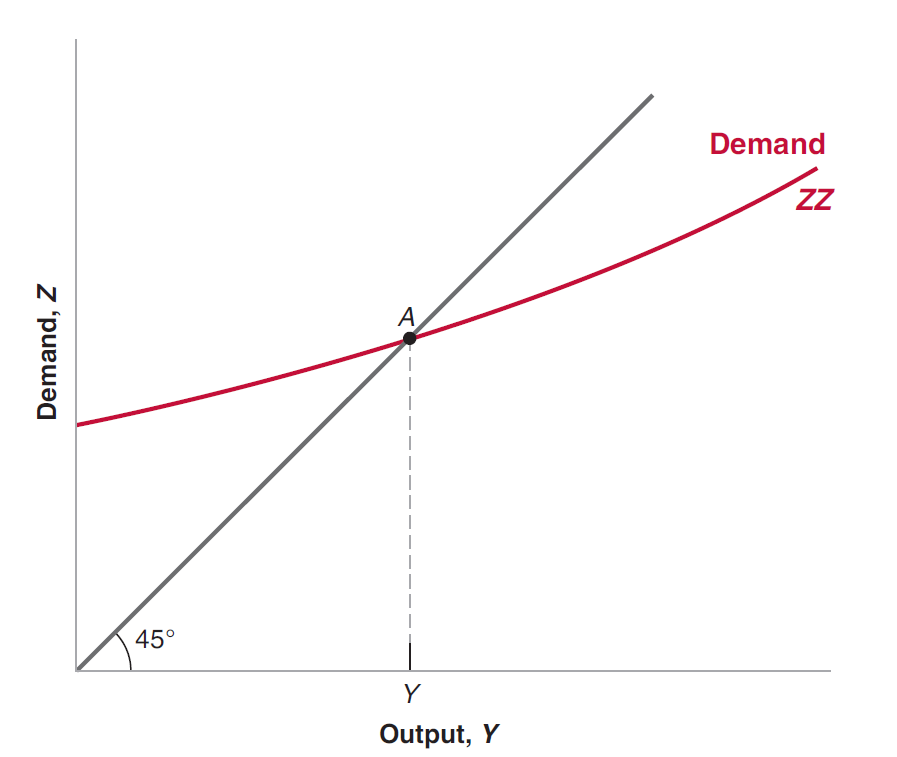
\includegraphics[width=1\textwidth]{5_1} %插入图片,[]中设置图片大小,{}中是图片文件名
	\caption{Equilibrium in the Goods
		Market} %最终文档中希望显示的图片标题
	\label{Fig.main2} %用于文内引用的标签
\end{figure}

我们没有假定,消费和投资是线性关系,所以ZZ线一般是曲线而不是直线。

ZZ线比$ 45^{\circ} $线平坦,也就是说我们假定产出增加,需求以小于1:1的比例增加。

\subsection{IS曲线的推导}
利率上升减少了投资,投资减少导致了产出减少,而产出的减少通过乘数效应进一步减少了消费和投资。

将利率与其均衡产出意义对应即得到IS曲线。(产出越高,均衡利率越低。)

\begin{figure}[H] %H为当前位置,!htb为忽略美学标准,htbp为浮动图形
	\centering %图片居中
	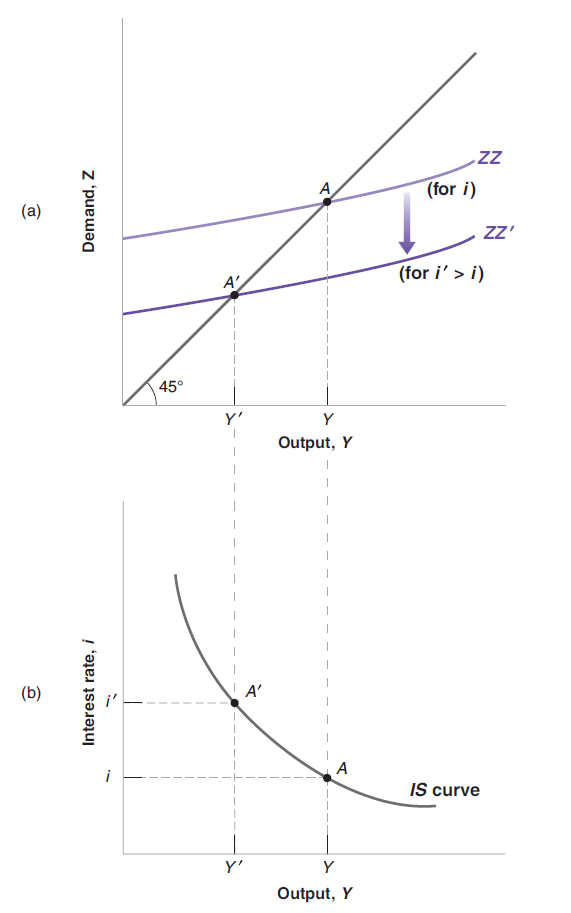
\includegraphics[width=1\textwidth]{5_2} %插入图片,[]中设置图片大小,{}中是图片文件名
	\caption{The IS Curve} %最终文档中希望显示的图片标题
	\label{Fig.main3} %用于文内引用的标签
\end{figure}


\subsection{IS曲线的移动(左右移动,因为IS关系是指各种因素对Y的影响)}
税收T的增加或政府支出G的减少会导致IS曲线左移,反之右移。(给定利率的情况下,任何减少均衡产出的因素都会导致均衡产出左移,反之右移。)
\[
Y=\frac{c_0-c_1T+G_0+I_0-bR}{1-c_1}
\]
$ c_0 $、$ I_0 $、$ G_0 $、$ T_0 $(固定税)

\hspace*{\fill}

比例税:$ T=T_0+tY $
\[
Y=c_0+G_0+I_0+c_1[Y-(T_0+tY)]-bR
\]
\[
[1-c_1(1-t)]Y=c_0+I_0+G_0-c_1T_0-bR
\]
\[
Y=\frac{c_0-c_1T_0+G_0+I_0-bR}{1-c_1(1-t)}
\]

投资需求的利率弹性b上升,IS曲线更平坦,反之反是;

税率t上升,IS曲线变陡峭,反之反是。

边际消费倾向$ c_1 $上升,IS曲线变平坦,反之反是。  


IS曲线越平坦,货币政策效力越大(t 减小,b上升,$ c_1 $上升)。

t减小,$ c_1 $上升,财政政策效力变大。(在LM平坦时不用考虑b?)

\section{金融市场和LM关系}
\[
M=\$YL(i)
\]
左边的M代表名义货币存量(认为中央银行直接控制M);右边代表货币需求(是名义收入和名义利率的关系)。

\subsection{实际货币、实际收入和利率}
将金融市场均衡等式两边同时除以价格水平:
\[
\frac{M}{P}=YL(i)
\]
因此,均衡条件也可以表达为实际货币供给(等式左边)等于实际货币需求(等式右边)(取决于实际收入Y和利率i)。

||此处利率为实际利率还是名义利率?||

\[
\frac{M}{P}=kY-hR
\]
h 为货币需求的利率弹性(h上升,LM曲线更平坦)

k 为货币需求的收入弹性(k上升,LM曲线更陡峭)
\subsection{LM曲线的推导}

以货币供给量为货币政策变量,传统的LM曲线推导方式:

给定收入水平,货币需求是利率的减函数。

收入增加导致在任何利率水平的货币需求都增加,货币需求曲线右移,当货币供给固定,均衡利率上升。

收入越高。对应的金融市场均衡利率越高。

\hspace*{\fill}

现实中央行通常以利率为货币政策目标,它选择利率水平$ \overline{i} $,进而通过调整货币供给水平以达到其所选择的利率水平。因此得到的LM曲线为一条处于中央银行选择的利率水平$ \overline{i} $下的水平线。

\begin{figure}[H] %H为当前位置,!htb为忽略美学标准,htbp为浮动图形
	\centering %图片居中
	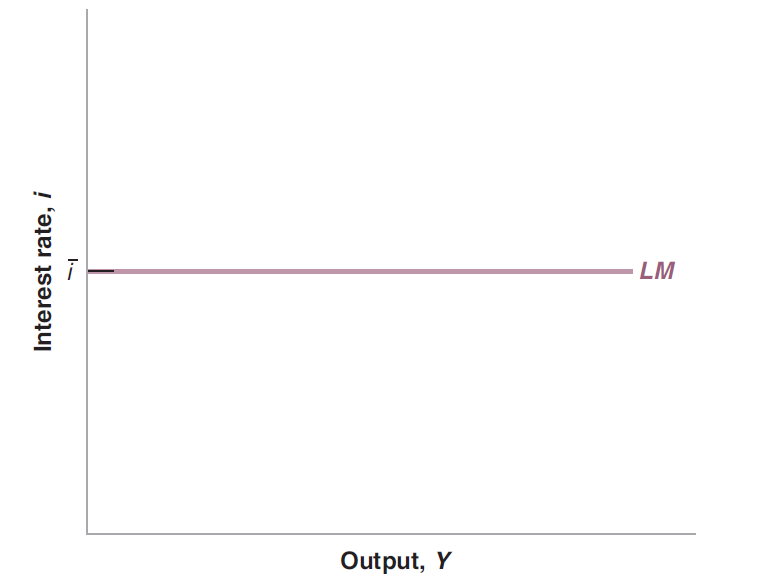
\includegraphics[width=1\textwidth]{5_3} %插入图片,[]中设置图片大小,{}中是图片文件名
	\caption{The LM Curve} %最终文档中希望显示的图片标题
	\label{Fig.main4} %用于文内引用的标签
\end{figure}

%\subsection{LM曲线的移动}
%实际货币供给$ M/P $的增加导致LM曲线下移,反之上移。

%\section{综合考虑IS关系和LM关系}
%IS关系表示在商品供给等于商品需求的条件下,利率是如何影响产出的。LM关系表示在货币供给等于货币需求的条件下,产出是如何影响利率的。
%IS关系和LM关系同时成立(产品市场和金融市场同时均衡):
%\[
%Y=C(Y-T)+I(Y,i)+G
%\]
%\[
%\frac{M}{P}=YL(i)
%\]

\section{IS-LM模型}

IS关系由产品供给等于产品需求的均衡条件得出。LM关系由金融市场均衡得出。它们必须同时成立。

IS关系:$ Y=C(Y-T)+I(Y,i)+G $

LM关系:$ i=\overline{i} $

\begin{figure}[H] %H为当前位置,!htb为忽略美学标准,htbp为浮动图形
	\centering %图片居中
	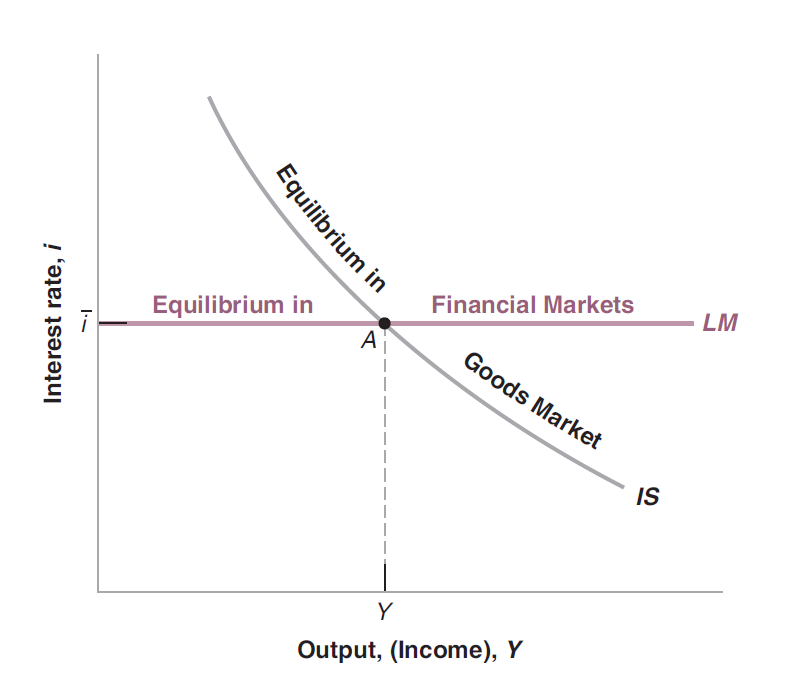
\includegraphics[width=1\textwidth]{5_4} %插入图片,[]中设置图片大小,{}中是图片文件名
	\caption{The IS-LM Model} %最终文档中希望显示的图片标题
	\label{Fig.main5} %用于文内引用的标签
\end{figure}







\iffalse
\subsection{财政政策、经济活动和利率}
税收增加$ \rightarrow $可支配收入减少$ \rightarrow $消费减少$ \rightarrow $产出和收入减少$ \rightarrow $货币需求减少$ \rightarrow $利率下降。

投资不确定(投资和销售水平以及利率二者有关,加税会导致可支配收入减少,再导致消费下降)。(若投资完全取决于利率则投资一定增加。)政府赤字增加导致投资减少叫作投资被赤字挤出;政府赤字增加导致投资增加叫作投资被赤字挤入。

\[
I=S+(T-G)
\]
若T增加的同时S(私人储蓄)减少且幅度大于(T-G)增加则I减少。换言之,财政紧缩可能导致投资下降。(反之财政扩张可能使投资增加)

G-T增加,财政扩张;
	w
G-T减少,财政紧缩

(动态调节!!!)

\subsection{货币政策、经济活动和利率}
货币供给增加称为货币扩张,货币供给减少称为货币紧缩。

货币扩张$ \rightarrow $利率下降$ \rightarrow $投资增加$ \rightarrow $需求和产出增加。

货币扩张后收入增加税收不变,可支配收入上升,消费上升;消费上升的同时利率下降,投资也增加。货币扩张政策比财政扩张政策对投资更有利。

Y为IS曲线(商品市场)的内生变量,R为LM曲线(货币市场)的内生变量

\section{使用政策组合}

\section{IS-LM模型与现实的吻合程度如何}
\fi





\subsection{财政政策}

G-T减少$\Leftrightarrow$财政紧缩;

G-T增加$\Leftrightarrow$财政扩张。

税收增加对产品市场均衡的影响——税收增加将带来产出的下降。IS曲线左移。
对金融市场的影响——由于中央银行没有调整利率。因此,LM曲线即$ i=\overline{i} $保持不变。LM曲线未移动。

均衡的决定。税收增加前,均衡由IS曲线和LM曲线的交点A给出。税收增加后,IS曲线向左移动,从IS曲线移动到$ IS' $,新的均衡点为$ A' $点。产出从Y下降到$ Y' $。

文字表述:

税收增加$ \rightarrow $可支配收入减少$ \rightarrow $消费减少$ \rightarrow $产出和收入减少。

给定利率水平下,税收增加导致产出下降。关于产出的构成:收入减少和税收增加都将导致可支配收入减少,进而导致消费减少。产出减少导致投资减少。从而,消费和投资都减少。

\begin{figure}[H] %H为当前位置,!htb为忽略美学标准,htbp为浮动图形
	\centering %图片居中
	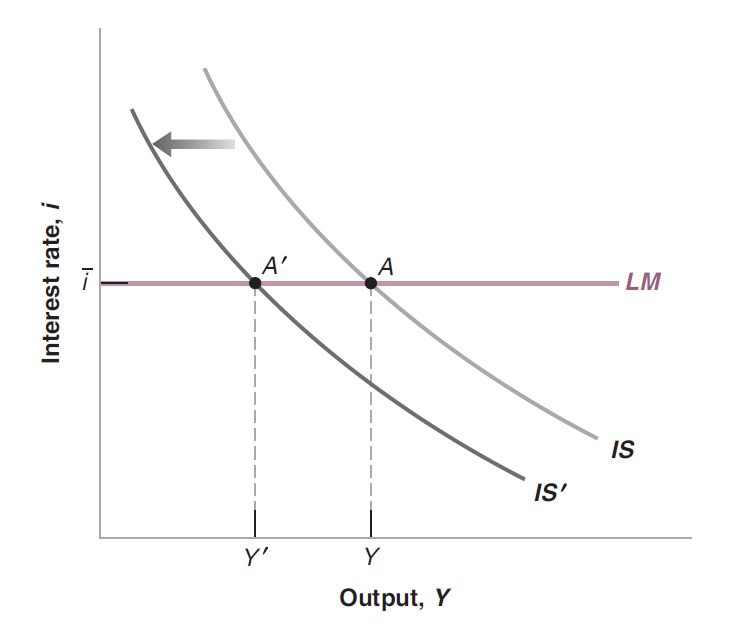
\includegraphics[width=1\textwidth]{5_5} %插入图片,[]中设置图片大小,{}中是图片文件名
	\caption{The Effects of an Increase
		in Taxes} %最终文档中希望显示的图片标题
	\label{Fig.main6} %用于文内引用的标签
\end{figure}

\subsection{货币政策}

货币扩张:中央银行通过增加货币供给来降低利率水平;

货币紧缩:中央银行减少货币供给。

i下降$\Leftrightarrow$M增加$\Leftrightarrow$货币扩张

i上升$\Leftrightarrow$M减少$\Leftrightarrow$货币紧缩

考察IS曲线和LM曲线是否移动:

IS曲线:利率水平的变化不直接影响产品的需求和供给。因此,i改变,IS曲线不会移动。

LM曲线:利率的水平变化将带来LM曲线的微小移动。LM曲线向下移动,从$ i=\overline{i} $处的水平线移动到$ i=\overline{i}' $。

均衡点从A移动到A'点。产出从Y增加到Y',利率从$ \overline{i} $下降到$ \overline{i}' $。

文字表述:利率下降导致投资增加,进一步导致需求和产出增加。在产出构成方面,产出增加和利率下降都带来投资的增加。收入增加带来可支配收入进而消费的增加。从而消费和投资都增加。

\begin{figure}[H] %H为当前位置,!htb为忽略美学标准,htbp为浮动图形
	\centering %图片居中
	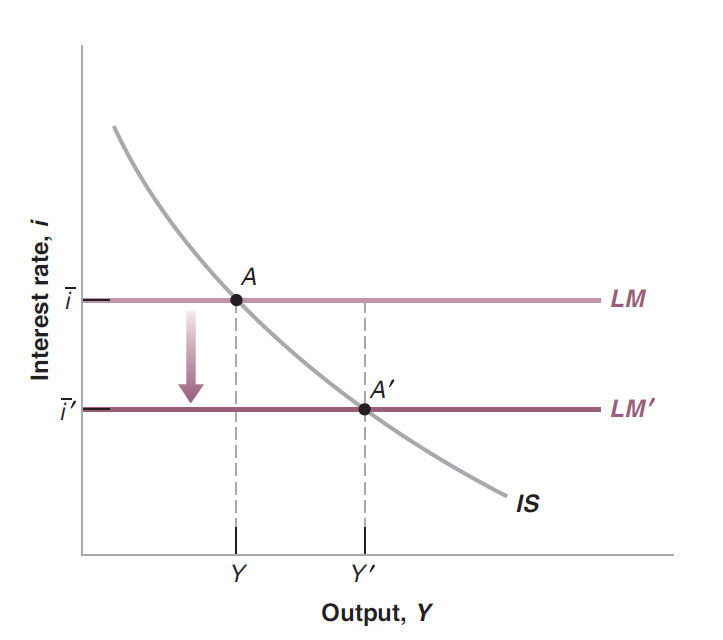
\includegraphics[width=1\textwidth]{5_6} %插入图片,[]中设置图片大小,{}中是图片文件名
	\caption{The Effects of a Decrease
		in the Interest Rate} %最终文档中希望显示的图片标题
	\label{Fig.main7} %用于文内引用的标签
\end{figure}

\section{政策组合}

财政扩张政策意味着政府支出的增加,或者税收的减少,或者二者兼有之。这意味着财政赤字的增加。财政严重赤字并增加政府负债可能是危险的。在这种情况下,至少部分通过货币政策来解决问题更佳。

货币扩张意味着利率下降。如果利率水平很低,那么使用货币政策的空间可能非常有限。在这种情况下。财政政策就需要发挥更大的作用。如果利率已经等于0,就得完全依靠财政政策。

财政政策和货币政策对产出的各个构成有着不同的影响。例如,收入税的下降带来的消费增加大于投资的增加。利率的下降对投资的影响大于其对消费的影响。因此政策制定者可能根据初始产出的构成来决定更多地运用财政政策还是货币政策。

财政政策或者货币政策都不是完美的。减税可能未能实现消费的增加。利率下降可能未能实现投资的增加。因此,如果一项政策未能达到预期效果,那么最好组合使用两项政策。

\begin{figure}[H] %H为当前位置,!htb为忽略美学标准,htbp为浮动图形
	\centering %图片居中
	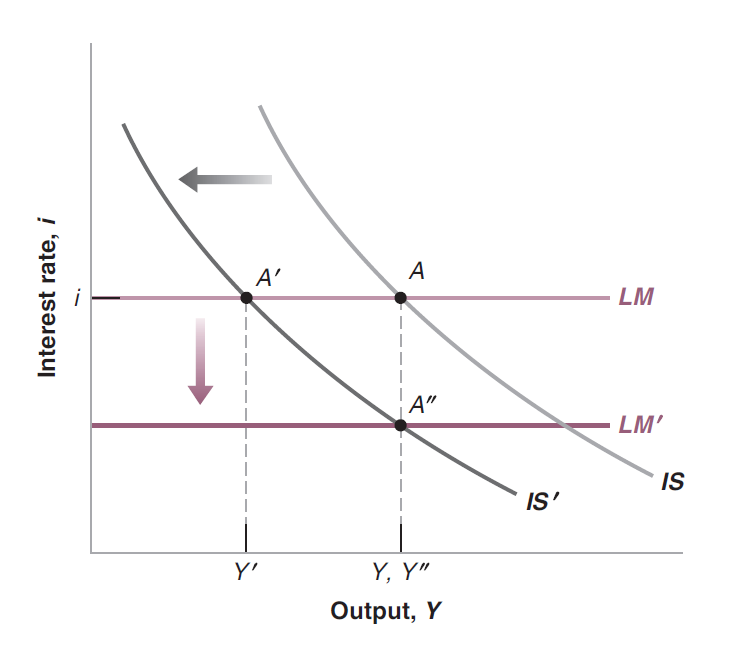
\includegraphics[width=1\textwidth]{5_7} %插入图片,[]中设置图片大小,{}中是图片文件名
	\caption{The Effects of a Combined
		Fiscal Consolidation and
		a Monetary Expansion} %最终文档中希望显示的图片标题
	\label{Fig.main8} %用于文内引用的标签
\end{figure}

在财政紧缩和货币扩张政策的组合效应下,消费的变化取决于赤字是如何减少的。如果是通过政府支出减少而非税收增加而实现的,那么收入将保持不变,可支配收入也保持不变,从而消费保持不变。如果是通过税收增加实现的,那么可支配收入减少,从而消费也将减少。投资变化则比较清楚:不变产出和较低的利率水平意味着较高的投资。

\hspace*{\fill}

赤字减少对投资来说是好还是坏:

产品市场均衡:

\[
I=S+(T-G)
\]

若给定私人储蓄如果政府减少赤字,投资必然增加:给定S,T-G增加,意味着I增加。

但给定私人储蓄这个假设不一定能成立。因为财政紧缩政策也会影响私人储蓄:紧缩导致较低的产出,进而导致较低的收入。消费的减少幅度小于收入,因此私人储蓄下降。事实上,私人储蓄的减少幅度大于财政赤字的减少幅度,从而导致投资减少。用等式表达即是:如果S减少的比T-G增加的多,那么I会减少。

但这也并不意味着赤字的减少总是会减少投资,如果赤字减少,中央银行为了维持产出水平保持不变,会同时降低利率,那么投资自然就增加了。尽管产出水平保持不变,但较低的利率水平带来了较高的投资水平。

总结。赤字减少对投资的影响不是确定的:可能是增加也可能不是,这取决于货币政策的反应。

P.S.:个人觉得若单纯使用财政政策(不配合货币政策),产出减少利率不变的条件下投资将减少。

\section{IS-LM模型和现实的关系}

现实:

在可支配收入改变后,消费者可能需要一段时间来调整消费。

在销售量改变后,企业可能需要一段时间来调整投资。

在利率改变后,企业可能需要一段时间来调整投资。

在销售量改变后,企业可能需要一段时间来调整产出。

\hspace*{\fill}

货币政策和财政政策改变后需要一段时间来调整产出。



\end{document}